\section{Montos de cotización}

\begin{wraptable}{r}{8cm}
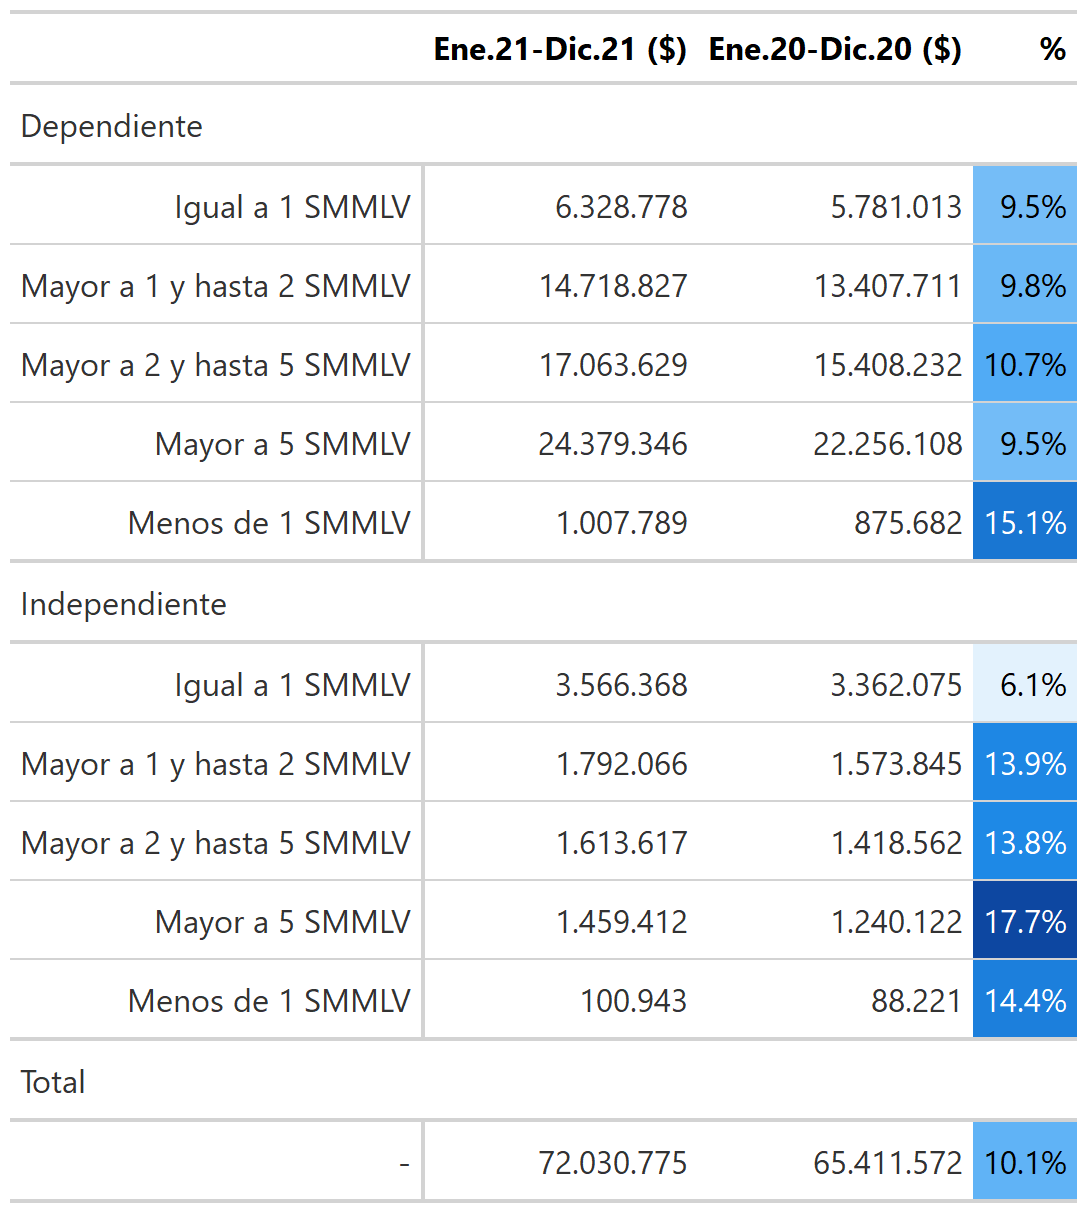
\includegraphics[width = 8cm]{results/03_financiero/salida_montos_cotizacion_interes_coomparativo.png}
\caption{Comparativo de montos acumulados en un periodo de 12
meses (Mill.)}
\label{tabla:montos:acumulados}
\end{wraptable}

El resultado presentado en la tabla \ref{tabla:montos:acumulados} muestra el comportamiento de 

\lipsum[2-4]


\begin{table}[!h]
\centering
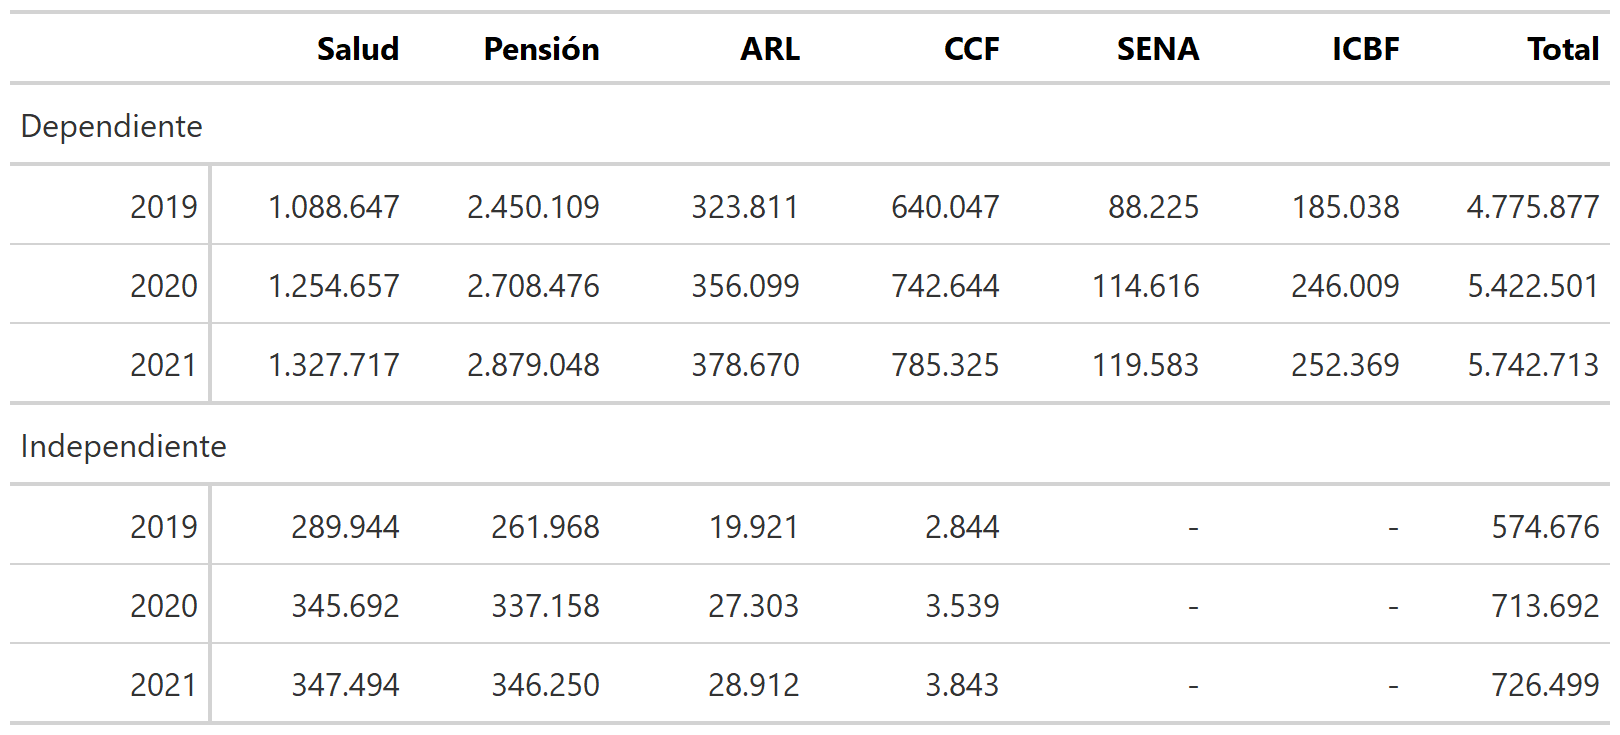
\includegraphics[width = 15cm]{results/03_financiero/salida_montos_cotizacion_subsistema.png}
\caption{Comparativo aportes por sub-sistema}%
\label{tabla:montos:sub_sistemas}
\end{table}



Solo pension--> Reemplazar tabla con gráfico (hablar con Juan Diego) 

incluir los montos a través de densidades de probabilidad. 


